
\documentclass{scrartcl} % KOMA Dokumentenklasse mit DIN-Papier als Standard
\usepackage[a4paper]{geometry} % Paket zur flexiblen Anpassung des Seitenlayouts
\savegeometry{default}
\usepackage[autooneside=false]{scrlayer-scrpage} % Paket zur flexiblen Anpassung der Kopf- und Fußzeilen
%
%\usepackage[tocindentauto]{tocstyle} % Paket zur flexiblen Anpassung der Formatierung des Inhaltsverzeichnisses (wird hier nur benötigt, weil einmalig die Nummerierung auf römische Zahlen umgestellt wurde)
 %\usetocstyle{KOMAlike}
%
\usepackage[english]{babel} % Sprachenpaket zur Anpassung der Standardausgaben von bestimmten Schlüsselwörtern und Aktivierung der deutschen Silbentrennung
%
\usepackage{miller}%to intuitively display miller indices%

\usepackage{parskip} %gets rid of hbox warning - just add empty lines to imply linebreaks

\usepackage[utf8]{inputenc} % Kodierungspaket zur Festlegung, wie die eingegebenen Zeichen (Code hier im Dokument) interpretiert werden sollen
%
\usepackage{csquotes}

\usepackage[T1]{fontenc} % Kodierungspaket zur Festlegung, wie die ausgegebenen Zeichen (Buchstaben im PDF-Dokument) implementiert werden sollen
%
\usepackage{lipsum} % Paket zur Einbindung von lateinischen Blindtexten
%
\usepackage{multicol} % Paket zur flexiblen Erstellung mehrspaltiger Texte und zum Zusammenfassen von Spalten in Tabellen
%
\usepackage{ragged2e} % Paket zur Verbesserung der Darstellung von linksbündigem, rechtsbündigem und zentriertem Text (erlaubt Silbentrennung)
%
\usepackage{quoting} % Paket zur ansprechenden Darstellung von Zitaten
%
\usepackage[marginal,norule]{footmisc} % Paket zur flexiblen Anpassung der Formatierung von Fußnoten
%
\usepackage{listings} % Paket zur vereinfachten Einbindung und zur ansprechenden Darstellung von Code in beliebigen Programmiersprachen
%
\usepackage[section, below]{placeins}
%\usepackage[section]{placeins}
%
%
\usepackage{microtype} % Paket zur Verbesserung der Mikro-Typographie durch Anpassung von Zeilenenden und sinnvollen Reduzierung von Silbentrennungen
\usepackage{lmodern} % Schriftenpaket für Latin Modern Schriften (beliebig skalierbare, richtig implementierte Vektorschriften)
%\renewcommand{\rmdefault}{lmss} %to use sans serif by default
\usepackage{textcomp} % Paket zur Erweiterung von verfügbaren Sonderzeichen (Copyright, Trademark, ...)
%
\usepackage{textgreek} %to use greek letters in text
%
\usepackage{amsmath} % Extrem umfassendes Mathematik-Paket der American Math Society
% allow for wider matrices
\newcommand{\tens}[1]{\boldsymbol{\mathsf{#1}}}
\setcounter{MaxMatrixCols}{20}
\usepackage{mathtools} % Erweiterung des amsmath-Pakets (enthält amsmath-Paket)
% Ergänzungen für Mathe:
\DeclarePairedDelimiter\abs{\lvert}{\rvert}%
\DeclarePairedDelimiter\norm{\lVert}{\rVert}%
%
%
% Anpassung von Klammern 
% Swap the definition of \abs* and \norm*, so that \abs
% and \norm resizes the size of the brackets, and the 
% starred version does not.
\makeatletter
\let\oldabs\abs
\def\abs{\@ifstar{\oldabs}{\oldabs*}}
%
\let\oldnorm\norm
\def\norm{\@ifstar{\oldnorm}{\oldnorm*}}
\makeatother
%
%
\usepackage{amsfonts} % Schriftenpaket der American Math Society zur Erweiterung der Schriften in Mathe-Umgebungen
%
\usepackage{amssymb} % Paket zur Erweiterung der verfügbaren Mathe-Symbole
%
\usepackage{MnSymbol} % Paket zur Erweiterung der verfügbaren Mathe-Symbole
%
\usepackage{graphicx} % Paket zur vereinfachten und flexiblen Einbindung von Grafiken (jpg, png, pdf)
%
\usepackage{pdfpages} % Paket zur vereinfachten und flexiblen Einbindung von mehrseitigen PDFs
%
\usepackage{chemformula} %Paket für chem. Formeln e.g. with \ce or \ch and stuff in brackets
%
\usepackage{xcolor} % Farbenpaket zur vereinfachten Einbindung und Anpassung von Farben
%
\usepackage{booktabs} % Paket zur Verbesserung der Darstellung von horizontalen Linien in Tabellen
%
\usepackage{multirow} % Paket zum Zusammenfassen von Zeilen in Tabellen
%
\usepackage{tikz} % Paket zur Erstellung von ansprechenden und anspruchsvollen Zeichnungen innerhalb von LaTeX
%\usepackage{pgfplots} % Paket zur Erstellung von ansprechenden und anspruchsvollen Plots innerhalb von LaTeX
%
\usepackage[style=nature, backend=biber]{biblatex} % Paket zur vereinfachten und automatisierten Erstellung eines Literaturverzeichnisses aus einer externen Datenbank

%
\usepackage{xparse} % Paket zur Erweiterung der Funktionalitäten bei der Definition von neuen Befehlen und Umgebungen
%
\usepackage{hyperref} % Paket zur Erstellung und Anpassung von anklickbaren, intelligenten Querverweisen innerhalb des Dokuments und Hyperlinks (Weblinks, Maillinks, Filelinks)
%
\def\code#1{\texttt{#1}} % to display cod in monospace using \code{arg1}
%
%
%
%
% Einstellungen für das Dokument:
%
 \KOMAoptions{headsepline, footsepline}
 \setkomafont{headsepline}{\color{gray}}
 \setkomafont{footsepline}{\color{gray}}
 \setkomafont{pagehead}{\scshape}
 \setkomafont{pagefoot}{} %\bfseries
 \automark[subsection]{section}
 \lohead{}
 \cohead{\rightmark}
 \rohead{}
 \lofoot{}
 \cofoot{\pagemark}
 \rofoot{}
%
%
\definecolor{meinSchwarz} {RGB} {0,0,0}
%
\hypersetup{linktoc = all, colorlinks ,  citecolor = meinSchwarz , linkcolor = blue, urlcolor  = meinSchwarz , filecolor = meinSchwarz }
%
%\addto\extrasngerman{\def\figureautorefname{Abb.}}
%
\setlength{\parindent}{0pt}
\setlength{\parskip}{0.5\baselineskip plus 0.2\baselineskip minus 0.1\baselineskip}
\linespread{1.25}
%
\newcommand{\degcel}{\,\textcelsius{} }
%
% Angaben zu Variablen
\graphicspath{{graphics}}
\bibliography{ddd_bib}
%

\begin{document}

%
\begin{titlepage}
\begin{center}

\includegraphics[width=0.5\textwidth]{graphics/FAU_TechFak_EN_H_black.eps}

\LARGE Department Materials Science

\Large WW8: Materials Simulation

\LARGE \textbf{Practical: Kinetic Monte Carlo Simulation}



\vfil
\Large Leon Pyka (22030137)



\Large \textbf{Supervision: Dr. Frank Wendler}
\end{center}

\thispagestyle{empty}
%
\end{titlepage}
%

\setcounter{page}{1}
\tableofcontents
\newpage

\section{Introduction}
The Monte Carlo method broadly refers to a large toolset of modelling methods utilizing the generation random numbers to solve problems. The underlying algorithm is the Metropolis algorithm. As opposed to Molecular Dynamics Monte Carlo methods do not follow the simulated particles trajectories over, but randomly perturbed the system to asses the the resulting systems properties in comparison to the preceding system. The  \textit{Kinetic Monte Carlo} (KMC) method incorporates kinetic features to the simulation. Each transition from state to state is seen is a diffusive jump and can happen at time-scales larger than in Molecular Dynamics (which is limited by the time-scale of atomic vibrations) \cite{voter2007}. 


\subsection{General Algorithm of the rejection free KMC Method}\label{sec:general_kmc_algorithm}

We start with a system of possible states \(i\) and possible transitions \(i \rightarrow j\). The transition rate is \(\nu_{ij}\). The following algorithm is reproduced from the problem statement \cite{zaiserb}.

\begin{enumerate}
	\item start with state \(i\) at time \(t\)
	\item evaluate total jump rate $\Gamma$ \begin{equation}
		\Gamma = \sum\limits_{j}\nu_{ij} \label{eq:total_jump_rate}
	\end{equation} 
	\item evaluate probability of jump by comparing \( \nu_{ij} \) to the total jump rate (eq. \ref{eq:jump_probability}) and calculate the cumulative probability \ref{eq:cumulative_probabilities} 
	\begin{subequations}
		\begin{align}
			p_{j} & = \frac{\nu_{ij}}{\Gamma} \label{eq:jump_probability} \\
			 P_{j }&= \sum\limits_{j'<j}p_{ij'} \label{eq:cumulative_probabilities}
		\end{align}
	\end{subequations} 
	\item generate a random number \(R_{1} \in [0,1)\)
	\item chose state which satisfies \( P_{ij} = \mathrm{min}{P_{il}, P_{il} > R_{1}}\) (where \(P_{il}\) is a list ordered in descending order, to make sure that high probability steps are more likely to be executed)
	\item generate random number \(R_{2} \in [0,1)\) and calculate jump time \(t_{ij}\) as
	\begin{equation}
		t_{ij} = - \frac{\ln(R_{2})}{\Gamma}
	\end{equation}
	\item update system configuration: \(i \rightarrow j\) and update time \(t = t + t_{ij}\)
	\item restart loop

\end{enumerate} 

\section{Diffusion Problems Solved with KMC}
\subsection{Diffusion in a Cu thin film with time dependent diffusion rate}
In this task we consider a sandwich structure of a Cu film and a Cu-10\% Al film, both of thickness 100~nm. As Cu is an fcc-metal it is possible to simplify the set-up to a 2D simple cubic lattice. The diffusion coefficient is given as:
\begin{equation}
	D = 1.49 \cdot 10^{-7} \exp \bigl( - \frac{136.1 \mathrm{kJ}}{\mathrm{R T}}   \bigr) \frac{\mathrm{m}^{2}}{\mathrm{s}}
\end{equation}

In 3D-the jump rate for e.g. Carbon at octahedral interstitial sites in $\alpha$-iron is given as \cite{gottstein2004}:

\begin{equation}
	\nu_{ij} = \frac{6D}{b^{2}}
\end{equation}

so for a 2D-simple cubic with 4 possible moving directions it should be given as:

\begin{equation}
	\nu_{ij} = \frac{6D}{b^{2}}
\end{equation}

The jump rate \(\nu_{ij}\) can be derived from D as follows:

\begin{equation}
	\nu_{ij} = \frac{4D}{b^{2}}
\end{equation}

with \(b = 2.54 \AA \). As we are considering only one kind of diffusion process \(\nu_{ij}\) is the same for all jumps so eq. \ref{eq:total_jump_rate} simplifies to:

\begin{equation}
	\Gamma = n \nu_{ij}
\end{equation}

and the probability from eq. \ref{eq:jump_probability} simplifies as stated below:

\begin{equation}
	p_{ij} = \frac{\nu_{ij}}{\Gamma} = \frac{1}{n}
\end{equation}

where \(n\) is the number of jumps. In the simulation the temperature needs to be increased linear to the time - from \(293~K\) to \(600~K\). So the temperature at every time step (after incrementation according to the algorithm in section \ref{sec:general_kmc_algorithm}) is found as:

\begin{equation}
	T_{i} = T_{\mathrm{start}} + \frac{T_{\mathrm{fin}} - T_{\mathrm{start}}}{t_{i}/t_{\mathrm{total}}}
\end{equation}

where \(T_{i}\) is the current temperature at time-step \(t_{i}\), \( T_{\mathrm{start}}\) is the initial temperature, \(T_{\mathrm{fin}}\) the temperature at the end and \(t_{\mathrm{total}}\) the total time until the heating is finished. 
Actually running the simulation exposes some additional challenges. As the size of the time-step is inversely proportional to \(\Gamma\). Meaning that the time-step at room temperature can become very large. So large indeed that it can exceed the total runtime of the simulation in the first step. To prevent this from happening the initially rejection free algorithm is updated to include the possibility of rejection. This is triggered when a certain time-step is exceeded. As the time and temperature are updated in the range of the time-step, but without performing a perturbation of the system. The second problem is the time-complexity of the simulation.  As we have to make sure that the system is updated after every move, to prevent e.g. Al atoms from switching sites with other Al-atoms. If this is checked for every jump the time complexity instantly becomes of size \(O(n^{2})\). This can be tackled, by using a data-frame storing both the atoms coordinates and their neighbors'. In the initial implementation a \code{pandas.DataFrame} was used. The random moving direction was chosen from the neighbors-list using the \code{pandas.sampel()} method. This resulted in a peculiar error - displayed in fig. \ref{fig:failed_implementation}. As all the  atoms seem to have a preferred moving direction this might expose a problem with the pseudo-randomness of the \code{pandas.sampel()} function. The tendency to choose the first moving direction (down) over the other direction shows that the the function seems not to be uniformly distributed, for the required sample size.

\begin{figure}[htb]
	\centering
	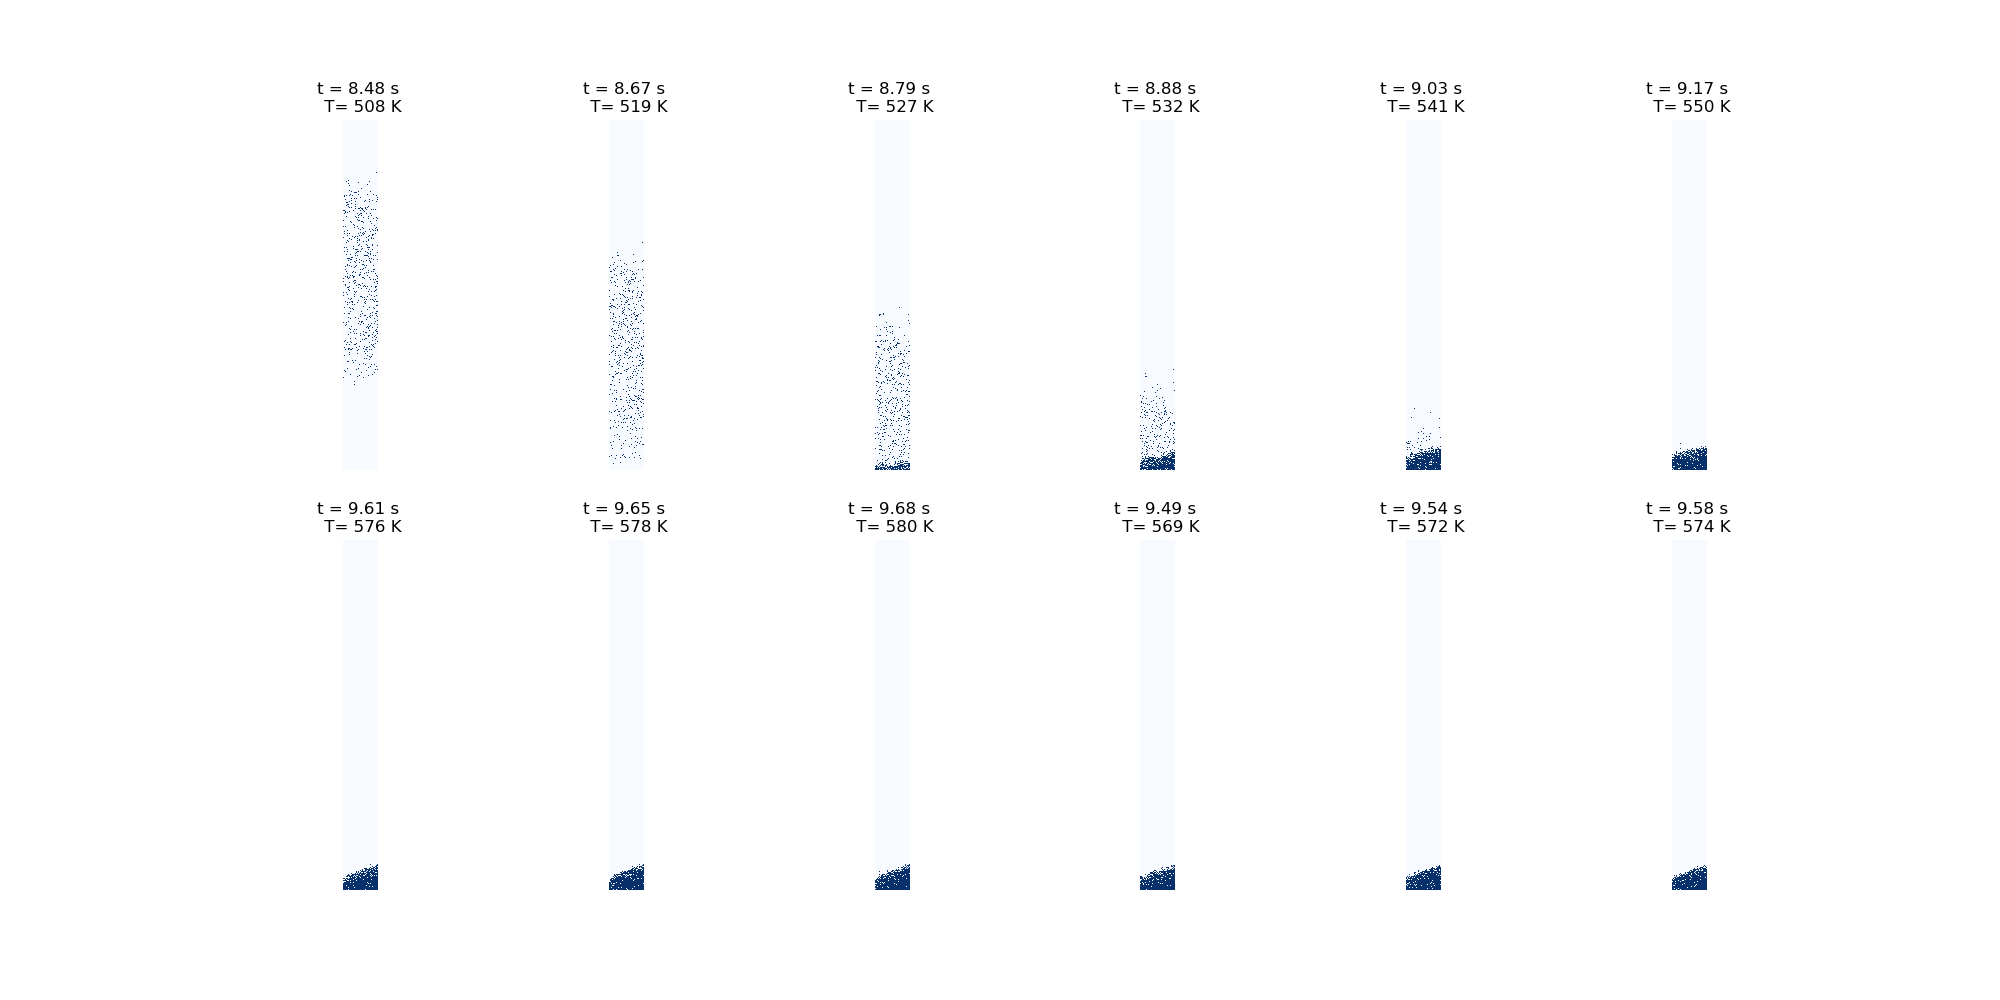
\includegraphics[width= \textwidth]{failed_implementation.png}\label{fig:failed_implementation}
	\caption{Failed implementation of diffusion in an Cu/Cu-10\% Al-sandwich structure. The blue dots represent Al-atoms at substitutional sites. }
\end{figure}

\begin{figure}[htb]
	\centering
	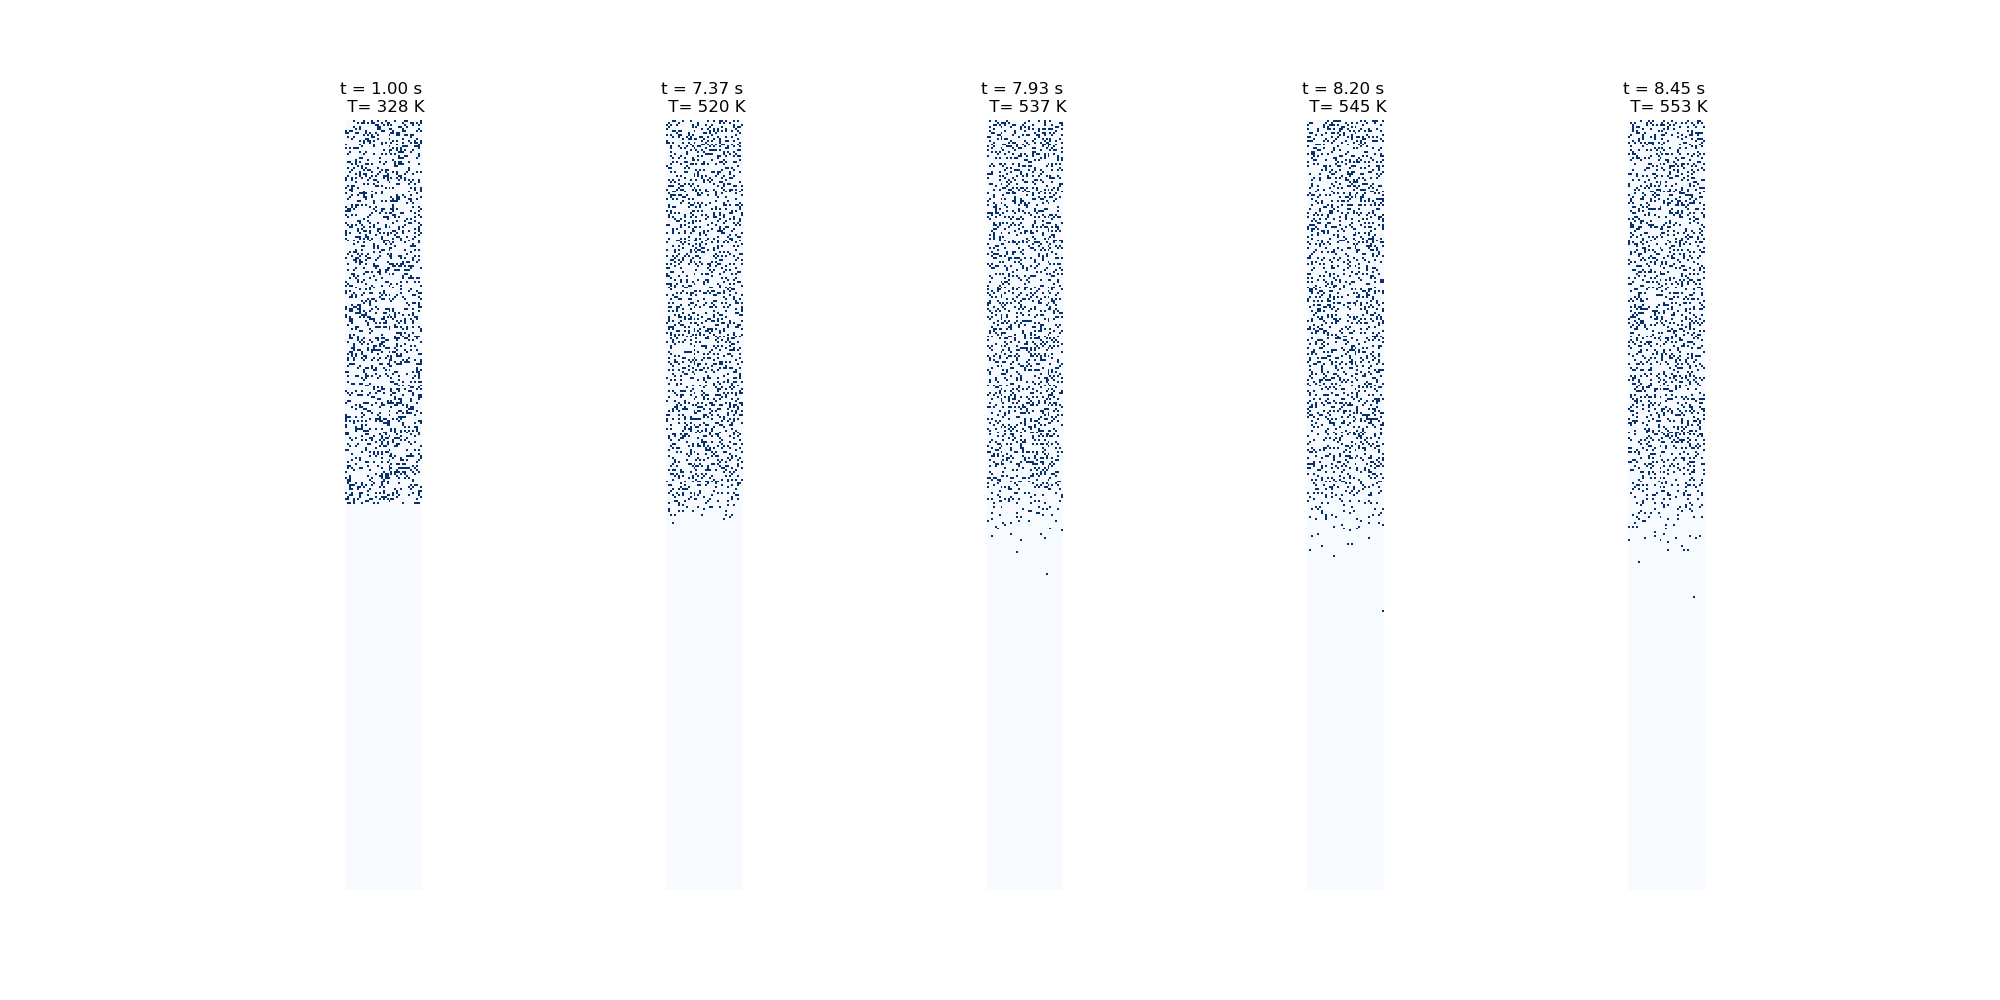
\includegraphics[width= \textwidth]{AlCu_01.png}\label{fig:Al_Cu_sandwich_time}
	\caption{KMC-Simulation of a Cu/Cu-10\% Al-sandwich structure. The blue dots represent Al-atoms at substitutional sites. }
\end{figure}

Fig. \ref{fig:Al_Cu_sandwich_time} shows a succesful implementation utilizing a \code{numpy.array} storing the individual atoms as objects carrying the type of the atom, the index of the neighboring atoms, the index of the sites with which the atom can switch places and the the number of switches the individual atom can perform. The flattening of the concentration gradient is qualitatively visible in fig. \ref{fig:alcu_time_concentration_plot}.

\begin{figure}[htb]
	\centering
	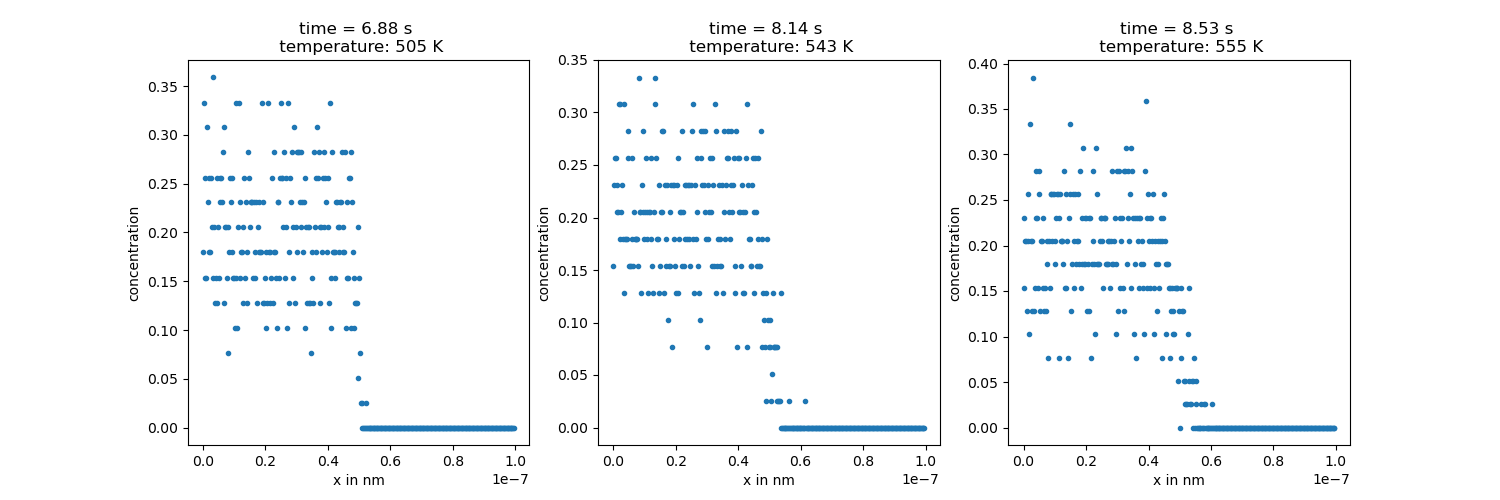
\includegraphics[width=\textwidth]{alcu_x_concentration_evolution.png}
	\caption{x-position against concentration of al per row at evaluated different times and temperatures. }
	\label{fig:alcu_time_concentration_plot}
\end{figure}


%\listoffigures
\printbibliography

\end{document}
